\documentclass{article}
\usepackage{ijcai13}
\usepackage{times}
\usepackage{latexsym} 

%\documentclass[letterpaper]{article}
%\usepackage{aaai}
%\usepackage{times}
%\usepackage{helvet}
%\usepackage{courier}
\usepackage{algorithm2e}
%\frenchspacing

\usepackage{graphicx}

\title{Social Computing Article\thanks{This title is temporary}}

\begin{document}

\maketitle

\begin{abstract}
Social collaboration has been shown to facilitate problem-solving activity in diverse sets of environments. Nevertheless, if not well designed, social and human computation systems may achieve results as poor as those of a single human subject performing a task. This scenario reflects a need for a better understanding of the performance issues of human problem-solving social networks. We present a novel method for artificial social problem solving and test it against results with human subjects, analysing which parameters have effects on the performance of problem-solving social networks. Results show that evaluating neighbours' solutions in order to decide from which neighbour to copy or mimic is significantly better than selecting solutions based on their position on the graphic interface, as tests with human subjects have shown to be the preferred behaviour among people. Our results also indicate that copying and guessing are highly beneficial to the performance of these social networks. We then use these results to propose a collection of guidelines concerning the design of a efficient human computation system.
\end{abstract}

\section{Introduction}

For years multi-agent systems have been used to research cooperation as a tool for problem-solving. %cite Malone
Recently, however, there has been an increasing interest in the study of human beings as problem-solving agents. Several experiments have been conducted in which subjects are connected in a network with the goal of collectively solving a specific problem, and those have helped shed some light on the way humans interact to solve problems as well as on the dynamics of working groups~\cite{woolley:evidencecollective}. However, although those studies can provide us with observations and hypotheses, there is still a difficulty in finding ways to explain the observed collective, human behaviour. In this paper, we use a multi-agent based simulation to complement %change?
the study of human computation, as a way of explaining the strategies used by humans when solving problems and understanding their consequences in a cooperative environment. The degree of control that simulations provide us over the behaviour of the agents allows us to better understand possible reasons for the actions and behaviours displayed by human agents.

Human beings are known to be able to easily perform tasks which are still generally difficult for computers, such as natural language processing and image recognition.
%--
However, it would be useful to apply human social computation to more straightforward computer problems with precise definitions and algorithms, but which are still computationally intensive.
%--
The different abilities of computers and humans suggest that the latter might provide a new approach to problems that might be more effective than current techniques employed by computers. That notion has been successfully applied, for example, in one of the most significant problems in the field of bioinformatics: protein structure prediction (PSP). A software that presents the problem to humans as an online computer game, called \emph{Foldit}~\cite{cooper:foldit}, has produced significant results in the research of PSP, which is usually approached as an optimization problem requiring extensive computational power. Such results have been attributed to human visual problem-solving and decision-making abilities, as well as social collaboration~\cite{cooper:foldit}. However, we still don't know the limits of human abilities in problem-solving and how they compare to more traditional computational techniques.
%--Exploit this point
In order to take full advantage of human problem-solving strategies, we must learn their limitations. Humans tend to be less efficient than computers in mathematical computations, are subject to a series of physical and psychological conditions that might affect their performance, and do not always act rationally.
We propose a model for simulating a problem-solving network of human agents. By applying in this model findings of experiments performed in humans, we can obtain knowledge about how human patterns of behaviour influence the problem-solving process. Through this system, it becomes possible to draw new conclusions from past observations of human behaviour. The model can be used, for example, to preview the results that changes in the infrastructure of a social computation system will have on its performance before actually performing the experiments with humans. Another possibility is to use the results obtained by the simulation of past experiments to plan the best configuration for a new system of social computing.
%--Move to Contribution?

\section{Background}

Human and social computing are relatively new areas of research with a diversified, interdisciplinary root that mixes social sciences, artificial intelligence, game theory and network science, among others. %cite ?, Kleinberg
Only recently studies on the potential of human social networks for solving problems are gaining some popularity. %cite Malone, Kearns
Those have provided insights into, among other things, the impact of network structure in the collaboration process and the factors that lead neighbours' proposed solutions to be copied by individuals.

The origin of human computation as we know it today can be traced back to the work of~\cite{vonahm:gwap}, which identified the possibility of using entertainment as an incentive to participation of human subjects, applying it in games in which the participants are actually performing a computation. That is an idea that also appears in the Foldit game. %cite

The series of experiments summarized in~\cite{kearns:experim} are among the first to try to take advantage of collective problem-solving abilities to solve classical computer problems. The experiments are mostly based on the concept of coordination: subjects have individual incentives that are expected to drive them to cooperate with one another and lead them toward the collective goal ~\cite{nowak:evolutioncooperation}.

Other initiatives have appeared, such as the ones by~\cite{farenzena:collabem} and~\cite{mason:collablearnet}, which take a different approach by having subjects trying to solve the collective problem individually, with the possibility of exchanging solutions between neighbours. Those have resulted in interesting conclusions on human behaviour when the possibility of copying peers is available. Our experiments follow this line of research.

The experiments conducted by~\cite{farenzena:collabem} had human beings trying to solve constraint satisfaction problems, namely Boolean Satisfiability (SAT)~\cite{cook:complexitytheoremproving} and the popular \emph{Sudoku} game~\cite{weber:satsudoku}, with individuals connected through the network being able to exchange partial solutions of the problem in question.
%--Make more specific
In that study a specific pattern of behaviour was observed which suggests that humans might not evaluate the solutions proposed by their peers, instead choosing the most readily available one.
%--
That behaviour is referred to as an evidence of conformism in human subjects. On the other hand,~\cite{mason:collablearnet} seem to suggest that their subjects did evaluate the available solutions, although %Unfortunately?
an in-depth analysis of that fact was not reported. That might mean that multiple factors might influence the behaviour of human agents. We analyse possible reasons for that in the \emph{Results} section. %We also analyse possible reasons for that behaviour in the \emph{Results} section.

\section{Contribution}

%--Keep?
We have developed and detailed a novel method for artificial social problem solving which draws inspiration from the {\em Memetic Networks} model proposed by~\cite{araujo:memenet}.
%--
It was then applied to build a multi-agent system that simulates the experiments of~\cite{farenzena:collabem}, using the model of human behaviour proposed by them. We limited our experiments to the {\em Sudoku} problem, which is more attractive and accessible to human beings while being NP-complete and equivalent to SAT. Through that process, we compared the problem-solving strategy %strategy?
typically used by humans with alternative, artificial strategies and reached the conclusion that it is detrimental to the problem-solving process.
%--Explain better
We verify that even an inaccurate metric of evaluation surpasses choosing an arbitrary neighbour to copy.
%--
In addition, we analyse the impact that copying and guessing have on the process of solving the problem. After obtaining those results, we are able to propose a set of guidelines for the design of social problem-solving systems that might address those issues and improve the performance of human computing.

\section{A Novel Method for %Artificial?
Social Problem Solving}
%P.S. method has two phases: communication and reasoning

A number of multi-agent methodologies that employ information flow through agents have been studied before. For instance, the {\em Memetic Networks} model proposed by~\cite{araujo:memenet} draws inspiration from the phenomenon of {\em Cultural Evolution} discussed by Dawkins in~\cite{dawkins:selfishgene} and has a network of agents sharing, copying and incrementing units of information in a similar way that nature, according to Dawkins, deals with {\em Memes}~\cite{dawkins:selfishgene}. Nevertheless, some aspects of social behaviour of great significance to social computing cannot be properly analysed through this methodologies. One example is the conformist behaviour studied in~\cite{cefferson:conformists} and~\cite{farenzena:collabem}. The proper study of these aspects demands a novel method for artificial collaborative problem solving.

We propose a method for solving computational problems by means of a network of agents endowed with social behaviour. Our algorithm is composed of an ordered set of $N$ agents, each encoding a partial solution to the problem, and a binary $N \times N$ matrix representing possible connections between agents. Additionally, our algorithm is composed of two stages, namely the {\em Social Stage} and the {\em Cognitive Stage}. %cite social psych

\begin{algorithm}
 \SetAlgoLined
 Initialize N agents, each encoding a partial solution to the problem\;
 \While{termination condition not met}
 {
 	\For{i = 1 to N}
 	{
 		\For{j = 1 to N}
 		{
 			\If{j is connected to i}
 			{
 				$A_{i}$ = $i_{th}$ agent\;
 				$A_{j}$ = $j_{th}$ agent\;
 				Add $A_{j}$'s solution to the collection of messages received by $A_{i}$\; %A.messages.add(j.solution)\;
 			}
 		}
 	}
 	\For{i = 1 to N} 
 	{
 		\CommentSty{ //Social Stage }\;
 		$A_{i}$ = $i_{th}$ agent\;
 		selectedMessage = select($A_{i}$.messages)\;
 		
 		\If{random(0,1) $<$ copyRate}
 		{
 			$A_{i}$.solution = selectedMessage\;
 		}
 	}
 	\For{i = 1 to N}
 	{
 		\CommentSty{ //Cognitive Stage }\;
 		$A_{i}$ = $i_{th}$ agent\;
 		Add local changes to $A_{i}$'s solution%$A_{i}$.solution = addLocalChanges($A_{i}$.solution)\;
 	}
 }
 \caption{Algorithm for the proposed model, encompassing the social and cognitive stages}
\end{algorithm}

\begin{itemize}
\item
Social Stage: In the {\em Social Stage}, messages are passed from agent to agent through the network connections. Agents are thus presented with a multiplicity of messages. There is a particular probability associated with the behaviour of agents choosing to copy one of these solutions in contrast to keeping their current solutions. We call this probability the {\em Copy Rate}. When an agent chooses to copy, he or she is then supposed to select for copying only one of his or her received messages. This is done by means of a particular message-selecting strategy.

\item
Cognitive Stage: In the {\em Cognitive Stage}, agents are supposed to add local changes to the messages copied in the previous stage. This is done by means of a heuristic or an exact method.
\end{itemize}

%--Change focus
\section{Performance Tests}
%--

In order to validate the algorithm as a social problem-solving technique, we have modelled the real-world collaborative {\em Sudoku} solving environment studied in~\cite{farenzena:collabem} through our method and tested it over a set of {\em Sudoku} instances, having in mind that the emergence of similar results as those observed by~\cite{farenzena:collabem} in their tests with {\em Sudoku} and {\em SAT} solving would validate our model as a good candidate for the design of social problem-solving simulations.

\subsection{Social Stage} %Generalize!

The experiments conducted by~\cite{farenzena:collabem} point out a series of observations about the dynamics of cooperation in problem solving with human beings. For instance, the authors analysis has shown that human subjects are more likely to engage in the behaviour of copying the most readily available solutions on the graphic interface than in that of evaluating the available solutions and choosing the best according to some criterion. We have modelled three message-selecting strategies to employ in the \emph{Social Stage}, where the first attempts to evaluate the solutions and choose the best one, the second mimics the human behaviour of selecting the first solutions with greater probability and the third simply picks a neighbour at random to copy.

\subsubsection{{\em Pick Most Filled} strategy}

This metric employs the intuitive strategy of selecting the most complete message for copying. In the specific case of {\em Sudoku} solving, this metric selects the most filled {\em Sudoku} partial solution. Put in other words, it selects the {\em Sudoku} partial solution with the least number of blank cells.

\subsubsection{{\em Pick Among First} strategy}

We know that, in some settings of collaborative problem-solving, human subjects are likely to copy the first (from left to right) solutions on the graphic interface~\cite{farenzena:collabem}. The authors have provided us with a mathematical model of this behaviour, stated as $\langle X(k)\rangle = (1-p)^{k-1}p$, where the parameter $p$ is fixed as $p = 0.5479$ and $\langle X(k)\rangle$ denotes the probability of an agent copying the $k_{th}$ neighbour solution.

We inserted this behaviour into our model by firstly generating a random ordering of neighbours for each agent in order to compose a simulated graphic interface. As a result, each agent visualizes some neighbours before or after others. Secondly, we translated the above mathematical model into a message-selecting metric in which the solution selected by an agent is the $k_{th}$ with probability $\langle X(k)\rangle$.

\subsubsection{{\em Pick Random} strategy}

This metric selects an arbitrary solution giving equal probability to each neighbour.

\subsection{Cognitive Stage}

{\em Sudoku} solving techniques are abundant in literature. %{\em Sudoku} strategy literature?
Those techniques are based on the reasoning usually employed by humans to solve \emph{Sudoku} puzzles. Davis~\cite{davis:mathsudoku} discusses a collection of these techniques, of which the {\em Naked Singles} rule, the {\em Hidden Singles} rule and the {\em Naked Twins} rule are some examples. These techniques intend to, given a partial {\em Sudoku} solution, generate a set of {\em movements} which can be used to mark cells of this {\em Sudoku} puzzle. We implemented $5$ of these rules, modelling each one of them as a function that maps a {\em Sudoku} partial solution to a set of {\em movements}. These functions can be used in the {\em Cognitive Stage} to add local changes to the {\em Sudoku} message received in the {\em Social Stage}.

The rules implemented were the {\em Unique Missing Candidate} rule, the {\em Naked Singles} rule, the {\em Hidden Singles} rule, the {\em Two out of Three} rule and the {\em Naked Twins} rule, all of which (with the exception of the {\em Two out of Three} rule) are discussed in~\cite{davis:mathsudoku}. In our modelling, each agent knows a particular quantity of rules, this quantity determining the agent's {\em level}. Our tests were all conducted with a heterogeneous population of agents of different {\em levels}. We detail below the 'two out of three' rule. For details on the other $4$ rules, see~\cite{davis:mathsudoku}.

\subsubsection{Two out of Three Rule}

This rule applies to groups of three contiguous $3 \times 3$ blocks. It aims to find a value $v$ such that $v$ is present in two of the three $3 \times 3$ blocks encompassed by the group, but missing on the third. It proceeds by enumerating all the candidate cells - namely the empty cells - on this block, and then, by eliminating from this set all the cells that are encompassed by the rows or columns in which $v$ is placed on the other two blocks. If the resulting set has cardinality $1$, the rule has successfully found a cell to mark.

\subsection{Copying Solutions}

In a study conducted by~\cite{farenzena:collabem}, subjects were invited to solve {\em Sudoku} puzzles and share them with other subjects with whom they were connected through a network topology. At any time, a player could copy solutions from one of his or her neighbours. The authors' analysis has shown that there is a different copy frequency associated with each topology. For instance, the scale free topology with $\gamma = 1.65$ resulted in a copy frequency of $87 \%$, while the fully connected topology resulted in a copy frequency of $42 \%$.

We incorporated this copying frequency into our modelling, recreating the scenario of the experiments conducted by~\cite{farenzena:collabem} by setting this parameter accordingly to the topologies we used.

\subsection{Guessing and Backtracking}

We have consistent evidence that trial-and-error is a part of the {\em Sudoku} solving experience. The need for trial-and-error in {\em Sudoku} puzzles is not a falsifiable conclusion, but a mathematical fact~\cite{davis:mathsudoku}. Some puzzles are only solvable by the means of a backtracking procedure.

In our modelling, we associate each agent with a numerical parameter determining the probability this agent has to guess when incapable of applying a typical {\em Sudoku} solving strategy.

Automatic {\em Sudoku} solvers employing a backtracking algorithm are easily programmed and very time-efficient. On the other hand, the space complexity of these algorithms is a barrier to most human solvers, who need to write down tons of observations in order to employ a backtracking strategy. With this in mind, we propose in our modelling a different kind of backtracking, intended to be more similar to the way human beings employ error correction in {\em Sudoku} solving in a collaborative environment such as the one analysed in~\cite{farenzena:collabem}, which we refer to as \emph{social backtracking}. In it, when faced with one or more conflicts in its own solution, an agent copies a solution from one of its neighbours. In our modelling, this is done by raising the copy rate of this particular agent to $1$.

\subsection{Network Topology}

We modelled our agent networks through the network topologies employed by~\cite{farenzena:collabem} in their tests with human social networks. The topologies used were the {\em fully connected} topology, the {\em scale free} topology~\cite{barabasi:linked}, the {\em ring-2} topology and the {\em ring-3} topology~\cite{newman:newtorks}.

\section{Results and Analysis}

We tested the above modelling using an heterogeneous, uniform agent distribution in which every agent {\em level} ($0$ to $5$) %explain; table?
had an equal representation in the population. We performed tests with varying values for the parameters of {\em copy rate}, {\em guess rate}, {\em message selecting metric} and {\em network topology}.

\subsection{A Novel Method For Simulating Human Problem-Solving Networks}

We have proposed a model based on social psychology to simulate human behaviour in a problem-solving social network. Through it, we can simulate previous experiments performed on humans by modelling the observed behaviour as the cognitive and social stages. That will allow us to examine the consequences of that behaviour without having to enlist human subjects, which is usually expensive and time-consuming~\cite{?}. Moreover this model can be used as a guide of what to look for in the data collected by the experiments, in which the strategies employed by the subjects to solve the problem individually are mapped into the cognitive stage and the metric employed to pick a neighbour to copy, into the social stage.

We have applied the model into one such human computing experiment and reached particular conclusions about the methods employed by humans on it. Since the same behaviour was observed for different problems, we can expect these results to be generalized to a certain class of problems and systems with specific characteristics. We provide further analysis and details below.

\begin{figure}
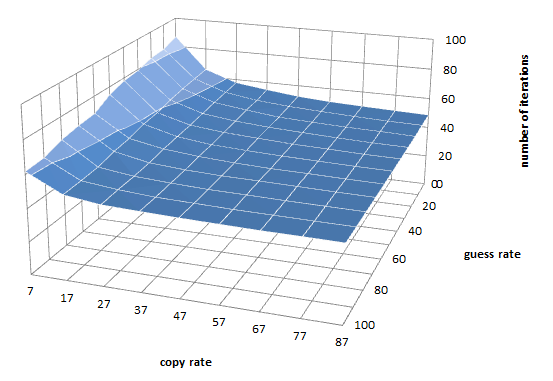
\includegraphics[scale=0.60]{copy_guess_free_most}
\caption{Effects of copy rate and guess rate on the algorithm's performance (scale-free topology with 'pick most filled' selection metric). The vertical axis represents the number of iterations needed for all the agents to find the correct solution.
}
\label{fig:copy_guess_free_most}
\end{figure}

\begin{figure}
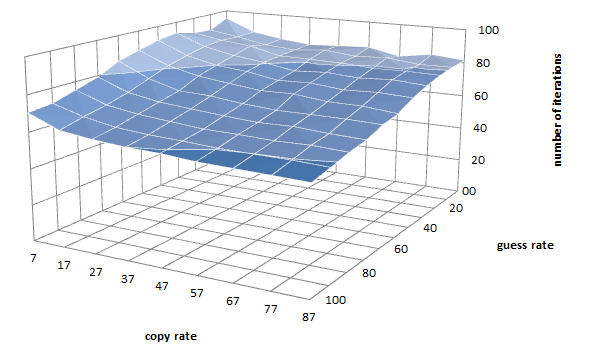
\includegraphics[scale=0.60]{copy_guess_free_prob}
\caption{Effects of copy rate and guess rate on the collective's problem solving performance (scale-free topology with 'pick among first' selection metric)
}
\label{fig:copy_guess_free_prob}
\end{figure}

\begin{figure}
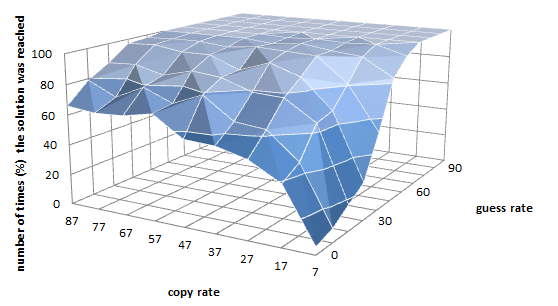
\includegraphics[scale=0.60]{copy_guess_free_prob_num_solution_reached}
\caption{Effects of copy rate and guess rate on the algorithm's convergence (scale-free topology with 'pick among first' selection metric)
}
\label{fig:copy_guess_free_prob_num_solution_reached}
\end{figure}

\subsection{Copying and Guessing are Beneficial to the Algorithm's Performance}

The authors of~\cite{farenzena:collabem} have stated that, in their settings, {\em "cooperation works because agents can copy each other"}. Basing ourselves in that statement, we adopted the hypothesis that a higher copy rate would improve performance of the network. On the other hand, regarding the process of guessing we took the opposite standing, that it would decrease performance. We based that hypothesis on the notion that, when an agent makes a guess, it has a high chance of filling a cell with the wrong value. Once that happens, that grid will assuredly be unable to lead to the right solution until the agent copies a grid without errors from one of its neighbours. Therefore, we hypothesised that if an agent can't make a logical move using its level of \emph{Sudoku}-solving skills, it's better for it to wait for its more capable neighbours to improve the solution and copy from them, instead of risking making and incorrect move.

Regarding our first hypothesis, our experiments indicate that, indeed, in some of the topologies tested, the {\em copy rate} has a decisive role in enhancing the network's performance. To our surprise, however, they also indicate that guessing shows no signs of being detrimental to the process. On the contrary, in several cases it actually contributes to advancing the solution. The graphs in Figure~\ref{fig:copy_guess_free_most} and Figure~\ref{fig:copy_guess_free_prob} both show a maximum in ({\em copy rate}: 7, {\em guess rate}: 0) and a minimum in ({\em copy rate}: 87, {\em guess rate}: 100), indicating that the greater the {\em copy} and {\em guess} rates are, the fewer rounds are needed for the agents to solve the problem. We understand this is due to the fact that some agents of low levels are incapable of solving some instances of the problem, not knowing the {\em Sudoku} solving rules needed to mark its cells. These agents have no hope solving the problem individually without some guessing mechanism, and the high {\em copy rates} allow them to correct wrong guesses through copying better agents' solutions.

The results also differ depending on the copying strategy employed in the \emph{social stage}. It can be observed that the copy rate has more influence over how fast the correct solution spreads through the network if the agents are evaluating their neighbour's solutions. The graph in Figure~\ref{fig:copy_guess_free_most} shows that as copying increases, the number of rounds necessary for all agents to have the correct solution decreases sharply until it stabilizes in a roughly optimal level. Meanwhile, the benefits of guessing are much less pronounced. On the other hand, when the agents don't evaluate the neighbours' solutions, as can be seen in Figure~\ref{fig:copy_guess_free_prob}, their contributions don't differ as much. Those results confirm that the worth of copying increases when the proposed solutions are evaluated.

Also, as shown in Figure~\ref{fig:copy_guess_free_prob_num_solution_reached}, there is a correlation between the copy and guess rates and the convergence of the algorithm: the greater they are, the greater is the probability that the agent network will be able to solve the problem.

\begin{figure}
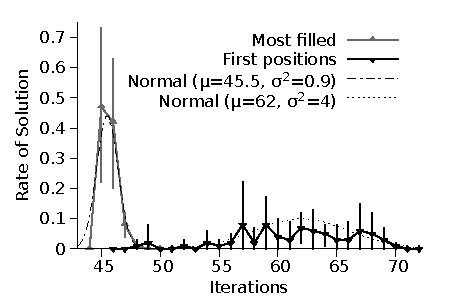
\includegraphics[scale=1]{ijcai_sudoku/ring}
\caption{Progression of the solution. The graph shows how many agents have successfully solved the puzzle in a given iteration (scale-free topology)}
\label{fig:ring_gauss}
\end{figure}

\begin{figure}
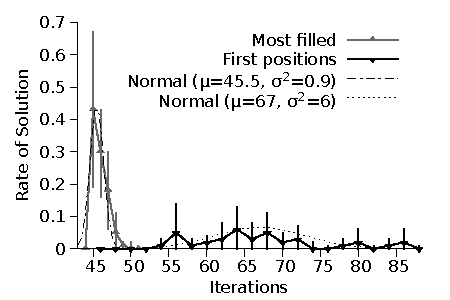
\includegraphics[scale=1]{ijcai_sudoku/sf}
\caption{Progression of the solution. The graph shows how many agents have successfully solved the puzzle in a given iteration (scale-free topology)}
\label{fig:sf_gauss}
\end{figure}

\begin{figure}
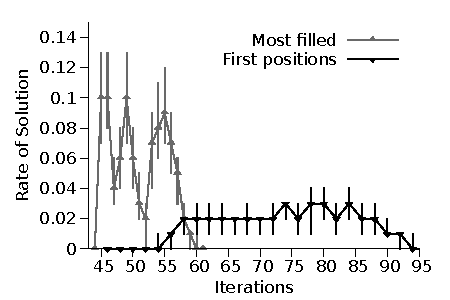
\includegraphics[scale=1]{ijcai_sudoku/geral}
\caption{Progression of the solution. The graph shows how many agents have successfully solved the puzzle in a given iteration (scale-free topology)}
\label{fig:global_gauss}
\end{figure}

\subsection{Evaluating Neighbours' Solutions is Advantageous even with an Inexact Metric}

Of the three metrics employed by us in the \emph{Social Stage}, only one had the agent evaluate the content of the solutions proposed by their neighbours. Another chose who to copy based on position, simulating observed human behaviour~\cite{farenzena:collabem}, and the remaining one chose a neighbour randomly. Our hypothesis was that the first metric would perform better than the other two, a result which would confirm our belief that problem-solving social networks respond positively to the employment of evaluation functions.

%%As can be seen in Figure~\ref{fig:progression}, 
Our experiments have shown that evaluating the proposed solutions indeed brings significantly better results, despite the fact that humans seemingly avoid that strategy~\cite{farenzena:collabem}. In all topologies, choosing the solution with the largest number of filled cells not only allows agents to solve the instance earlier, but also causes the network to converge faster to the correct solution. That is, once one individual has found the correct solution, that solution spreads faster through the network if the other agents are evaluating the solutions that reach them instead of copying an arbitrary one.

The strategy based on the behaviour observed in humans fared roughly the same as choosing a random neighbour to copy. That is to be expected because the position of each neighbour is already randomized, so there is virtually no difference between picking one of the first neighbours to copy and a random one among all. Seeing as the same conclusions apply to both the human and random strategies, we omit further analysis of the latter for simplicity. Both underperformed in comparison to evaluating the solutions according to number of filled cells. This confirms that choosing solutions arbitrarily without taking their content into consideration is prejudicial to the process of social problem-solving. 

We have observed in our experiments that the progress of the solution, represented by the number of agents that solve the problem in a given round, follows a normal distribution. During the first few rounds no agents have found the solution. Then, in a moment that varies according to the particular instance of the problem, the first few agents solve the problem. From that point onwards the solution starts spreading through the network. As more agents obtain the complete solution, more likely it becomes that further agents will copy that solution from their neighbours, according to the conformist behaviour observed in~\cite{farenzena:collabem}. That leads the number of agents to obtain the solution to progressively increase in the following rounds, until it reaches a point where the few remaining agents take longer to obtain the solution due to factors such as being less capable solvers or being in unfavourable positions in the topology.

We have run experiments in the four different topologies enumerated above, for 7 different problem instances, and obtained similar results in each. The progression of the solution for the \emph{Most Filled} and \emph{First Positions} strategies can be described as normal distributions of different mean and variance. In the context of the experiments, the mean indicates how soon the correct solution was found, and the variance how long it took to spread through the network. The exact values for those parameters vary widely according to factors such as topology and problem instance, but they follow a particular pattern. For all cases, the strategy that evaluated solutions had lower mean, indicating the solution was found sooner, and lower variance, meaning it spread faster. We have chosen the scale-free and 3-ring topologies as representative examples, and plotted the average of the results for a same instance of the problem for each in Figures~\ref{fig:sf_gauss} and~\ref{fig:ring_gauss}, respectively. In each can be seen the percentage of agents that find the correct solution in each round for the two strategies, with normal curves plotted over the values, evidencing the described behaviour. It's noticeable that the results fluctuate more for the second strategy, which is explained by its practically random method of choosing solutions to copy.

In Figure~\ref{fig:global_gauss} the average for all experiments can be seen, encompassing every topology and instance. In this graph, the presence of the normal behaviour in the distribution is less clear, due to it combining several different instances and topologies. Nevertheless, its effects can still be seen. The \emph{Most Filled} strategy displays different residual peaks from particular instances, while the line for the \emph{First Positions} strategy starts flattening with the accumulation of several distributions from the individual experiments. Most importantly, the general result of a sooner finding and faster spreading of the correct solution for the first strategy endures, showing its consistency over different scenarios.

Still, even though choosing a solution based on position instead of content is provably inefficient, that behaviour has been observed in human networks. In~\cite{farenzena:collabem} the authors suggest that it is justified in the real world because ``in a non-virtual environment, the feedback of the environment can cause an agent to stop communicating, e.g. in the case of injury or death'', so there would be no need for an agent to evaluate solutions because the environment is already selecting against ineffective ones. Since neither the original experiments nor our simulation included such a mechanism of natural selection, the advantages of that process have not been observed, but they might already be good enough that it would be unnecessary for the agents to have to spend effort evaluating the solutions.

Another explanation might be that humans might find difficult evaluating sudoku partial solutions. Although we have used the number of filled cells as a metric, that is not guaranteed to accurately measure which solution is best, since individuals might fill in cells with the wrong value. That hypothesis is supported by the experiments of~\cite{mason:collablearnet}, which used optimization of a bidimensional function as the problem being solved. This problem has a straightforward and accurate method of determining the fitness of a solution, which is simply the value of the given function for the proposed coordinates. In this experiments, the subjects seemingly did effectively evaluate the proposed solutions, giving preference to the ones that were better evaluated. The difference in behaviour between the two experiments might be because in the latter the fitness of a certain solution was obvious to the agent, while in the former it's not as easy to pick the best solution out of the available ones.

Our experiments, however, have shown that although completeness is not necessarily an accurate measurement of quality, it was good enough to lead the network to the right solution. Not only that, it consistently performed better than the other strategies, even with high guess rates.
%--Explain
That means that the incorrect guesses were successfully filtered out, allowing the correct solutions to prevail.
%--
Those results might extend to other constraint satisfaction problems that don't have an accurate method of evaluation. Therefore, it is not necessary for the problem addressed to have an exact metric to compare different possible solutions. An imperfect metric is good enough to be employed in a problem-solving social network. 

Also,~\cite{mason:collablearnet} differed in that each player had exactly three neighbours. That fact allowed the players to see all of their neighbours at the same time in the interface, and limit their attention to less data.~\cite{farenzena:collabem} suggests that future experiments might prefer to limit their topology to smaller degrees, seeing as subjects tend to not look beyond their first few neighbours. It is possible for the large number of neighbours to have discouraged an in-depth evaluation of the solutions by the players.

\subsection{Small Changes on the Interface Might Improve the Performance of Human Beings in Human Computation Environments}

Considering the previous results, systems of human computation might take advantage of the interface to encourage selection of better-evaluated solutions. One possibility is to display the evaluation of each solution to encourage players to copy the ones with better score. However, the SAT experiments from~\cite{farenzena:collabem} actually assigned a score to each solution displayed to the users, who nevertheless chose according to position rather than evaluation. Another possibility is ordering the neighbours according to the quality of their solutions, with better-evaluated ones being displayed first, instead of using a pre-specified or random order.

The limitation on the network's degree suggested by~\cite{farenzena:collabem} and employed by~\cite{mason:collablearnet} is also promising, and displays evidence of success. Fewer connections allows for all neighbours to be displayed in the interface at once, without necessity of effort by the user by clicking buttons or scrolling. Moreover, humans might feel more encouraged to evaluate their neighbours if the number of possible solutions is limited.
%
%\begin{figure}
%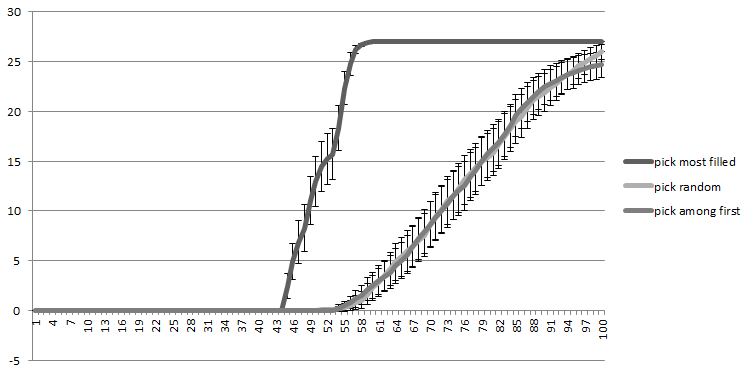
\includegraphics[scale=0.45]{progression}
%\caption{Progression of the solution. The graph shows how many agents have successfully solved the puzzle in a given iteration (scale-free topology)
%}
%\label{fig:progression}
%\end{figure}

\section{Conclusions and Further Work}
%"An interesting, unexpected result... (filtered)"
%Swap first two sentences

We compared results from social computing experiments done with human subjects with agent-based simulations mimicking the same problem-solving environments. To do this, we proposed a novel method for artificial social problem-solving and used it to model the {\em Sudoku} problem-solving environment studied by~\cite{farenzena:collabem}. We reached important conclusions concerning the dynamics of problem-solving collaborative environments: the behaviours of copying and guessing are shown to be beneficial to these systems. We also discuss the benefits of the behaviour of evaluating neighbours' solutions in order to select one of them for copying, rather than simply selecting a random solution or even the most readily available one, as the analysis conducted by~\cite{farenzena:collabem} has shown to be the case sometimes. With these results in mind, we conjectured that some properties of the graphic interface (as ordering the neighbours' solutions by the value of a evaluation function) could guide human subjects into the right direction, improving the performance of the social network. The validation of this hypothesis has been set as our future path and is currently being pursued.

%% The file named.bst is a bibliography style file for BibTeX 0.99c
\bibliographystyle{named}
\bibliography{Article}

\end{document}

